
\documentclass[
	article,
	12pt,				
	oneside,
	a4paper,
	english,
	brazil
]{abntex2}


% Configuracoes de fonte
\usepackage{helvet}	
\renewcommand{\familydefault}{\sfdefault}		
\usepackage[utf8]{inputenc}
\usepackage[T1]{fontenc}		

\renewcommand{\ABNTEXchapterfontsize}{\LARGE} % Tamanho dos títulos dos capítulos

% Pacotes fundamentais 
\usepackage{indentfirst}		
\usepackage{color}				
\usepackage{graphicx}			
\usepackage{microtype} 
\usepackage{pucmg}	% Customizacoes para os padroes PUC-MG
% ---

% Pacotes de citações
\usepackage[brazilian,hyperpageref]{backref}	 
\usepackage[alf,abnt-emphasize=bf]{abntex2cite}	% Citações padrão ABNT

% Informações de dados para CAPA e FOLHA DE ROSTO
\titulo{\Large{CLASSIFICAÇÃO DE SEGMENTOS EM ATOS NORMATIVOS ATRAVÉS DE PROCESSAMENTO DE LINGUAGEM NATURAL}}
\autor{Leandro Coelho Correia}
\local{Salvador}
\data{2021}
\instituicao{Pontifícia Universidade Católica de Minas Gerais}
\departamento{Núcleo de Educação à Distância}
\filiacao{Pós-graduação em Inteligência Artificial e Aprendizado de Máquina}
\tipotrabalho{Relatório técnico}
\preambulo{Trabalho de Conclusão de Curso apresentado ao Curso de Especialização em Inteligência Artificial e Aprendizado de Máquina como requisito parcial à obtenção do título de especialista.}
% ---

% informações do PDF
\makeatletter
\hypersetup{
     	%pagebackref=true,
		pdftitle={\@title}, 
		pdfauthor={\@author},
    	pdfsubject={\imprimirpreambulo},
	    pdfcreator={LaTeX with abnTeX2},
		pdfkeywords={abnt}{latex}{abntex}{abntex2}{relatório técnico}, 
		bookmarksdepth=4
}
\makeatother
% --- 

% Espaçamentos
\setlength\afterchapskip{12pt} % Após o título dos capítulos
\setlength\beforesecskip{12pt} % Antes do título das seções
\setlength\aftersecskip{12pt} 	% Após o título das seções
\setlength{\parindent}{1.3cm} 	% Identação da primeira linha do parágrafo
\setlength{\parskip}{0.2cm}  	% Espaçamento entre um parágrafo e outro

% Compila o índice
\makeindex


% Início do documento
\begin{document}

\selectlanguage{brazil}

% Retira espaço extra obsoleto entre as frases.
\frenchspacing 

% ----------------------------------------------------------
% ELEMENTOS PRÉ-TEXTUAIS
% ----------------------------------------------------------
\pretextual

\imprimircapa
\imprimirfolhaderosto*

% inserir lista de ilustrações
\pdfbookmark[0]{\listfigurename}{lof}
\listoffigures*
\cleardoublepage
% ---

% inserir lista de tabelas
\pdfbookmark[0]{\listtablename}{lot}
\listoftables*
\cleardoublepage
% ---

% ---
% inserir o sumario
% ---
\pdfbookmark[0]{\contentsname}{toc}
\tableofcontents*
\cleardoublepage
% ---

% ------------------
% ELEMENTOS TEXTUAIS
% ------------------
\textual

\begingroup
\let\clearpage\relax
\section{Introdução}

\subsection{Atos Normativos}

A publicação de atos normativos é uma etapa fundamental do processo de gestão pública, pois formaliza e divulga para a sociedade as decisões do Governo Federal. A Receita Federal do Brasil (RFB) disponibiliza atos normativos através do sistema Normas \cite{Normas2021}, acessível publicamente através da Internet. Os atos são inicialmente publicados no Diário Oficial da União (DOU) através da Imprensa Nacional \cite{ImprensaNacional2021} e incluídos manualmente no sistema Normas.

Um ato normativo é composto por segmentos, trechos que possuem um significado próprio definido pelo Decreto N\textsuperscript{o} 10.139 de 28 de novembro de 2019 \cite{Decreto10139} e formatação específica definida pelo Manual de Redação da Presidência de República \cite{ManualRedacao2018}. A figura \ref{fig:segmentos} apresenta um ato normativo destacando alguns segmentos de tipos diferentes: a ementa destacada em vermelho, um segmento não identificado destacado em azul, alguns artigos em verde e o fecho em marrom ao final do ato. 

\begin{figure}[h]
	\caption{Exemplo de ato normativo com segmentos em destaque}
	\center
	\label{fig:segmentos}
	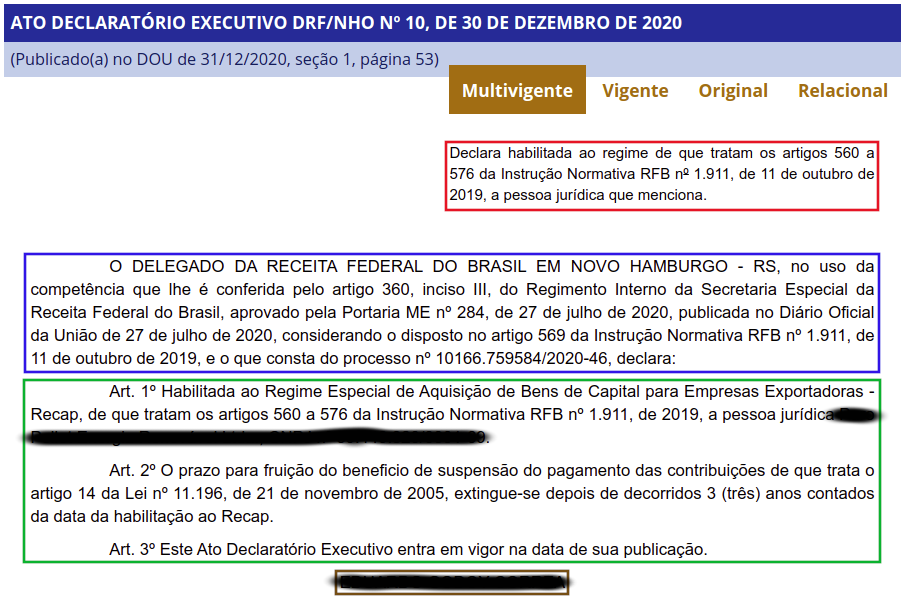
\includegraphics[scale=1.9]{introducao/segmentos.png}
	\fol{Normas2021}
\end{figure}

A classificação dos segmentos é uma etapa fundamental para o processo de inclusão de atos no sistema Normas, mas atualmente é realizada de forma totalmente manual, através de um procedimento que exige atenção e dedicação diária de uma equipe especializada da RFB. No período entre 2013 e 2020 foram incluídos aproximadamente 65 mil atos normativos compostos por mais de 600 mil segmentos, evidenciando um trabalho grande de classificação.

\subsection{Processamento de Linguagem Natural}

O Processamento de Linguagem Natural (PLN) é uma área da Ciência da Computação, fortemente relacionada com outras áreas de conhecimento como a Inteligência Artificial e o Aprendizado de Máquina, que pesquisa métodos para analisar, modelar e compreender a linguagem humana \cite{PracticalNLP2020}. Uma das tarefas de PLN é a classificação de textos que consiste em atribuir uma classe previamente conhecida a um texto informado. Alguns exemplos de classificação de textos são a identificação de \textit{spam} em mensagens eletrônicas e a análise de sentimentos em comentários de redes sociais. Para o escopo desta pesquisa os textos são os segmentos dos atos normativos e as classes são os diferentes tipos de segmento a exemplo da ementa, dos artigos, do fecho e do segmento não identificado mencionados anteriormente. 

\subsection{O Problema Proposto}

Este trabalho propôs a criação de um modelo de aprendizado de máquina, baseado em PLN, capaz de classificar automaticamente os segmentos de atos normativos provenientes do DOU, reduzindo o esforço e o tempo de inclusão dos atos no sistema Normas. A classificação automática de segmentos, além de contribuir para a otimização do trabalho da RFB, possibilita que os atos normativos sejam disponibilizados à sociedade em um intervalo de tempo menor.

Não fazem parte do escopo desta pesquisa a classificação do ato como um todo (pois o tipo do ato pode ser deduzido a partir do seu título através de heurísticas simples) nem o estudo dos relacionamentos entre os atos (uma funcionalidade complexa do sistema Normas que demanda uma pesquisa dedicada).

Para o desenvolvimento da pesquisa foi utilizada a linguagem de programação Python. A maior parte do código foi organizado em arquivos *.py contendo a lógica para realização das diversas etapas do fluxo de aprendizado de máquina. Além disso, foram criados dois Jupyter Notebooks responsáveis respectivamente pela realização da análise exploratória de dados e  orquestração das etapas do fluxo de aprendizado de máquina. Todo o código-fonte está disponível no repositório da pesquisa no Github\footnote{Segmentador Automático de Atos Normativos. Disponível em: \url{https://github.com/correialc/saan}. As versões das bibliotecas de software utilizadas estão descritas no arquivo \textit{requirements.txt} presente no repositório.}.





\section{Coleta de Dados}

Para a realização deste trabalho foi utilizado um conjunto de dados contendo 260.488 segmentos pertencentes a 20.821 atos do sistema Normas\footnote{Nem todos os atos do sistema Normas são de domínio público, mas todos os atos utilizados nesta pesquisa são públicos e podem ser acessados através da Internet, tanto pela Imprensa Nacional quanto pelo sistema Normas.}, relativos ao período de 01/01/2018 a 31/12/2020. Os dados estão em formato *.csv (arquivo extracacao-segmentos-atos.csv) e seguem a estrutura descrita na tabela \ref{tab:estrutura-conjunto-dados}.

\begin{table}[h!] 
\caption{Estrutura do conjunto de dados}
\label{tab:estrutura-conjunto-dados}
	\begin{center} 
		\begin{tabular}{|l|l|l|} 
			\hline ATRIBUTO & DESCRIÇÃO & TIPO \\
			\hline
			\hline id\textunderscore ato & Identificador do ato & Quantitativo Discreto \\ 
			\hline data\textunderscore  pub & Data de publicação do ato & Categórico Nominal \\ 
			\hline tipo\textunderscore  ato & Tipo do ato & Categórico Nominal \\
			\hline id\textunderscore seg & Identificador do segmento & Quantitativo Discreto \\
			\hline tipo\textunderscore seg & Tipo do segmento & Categórico Nominal \\
			\hline txt\textunderscore seg & Texto do segmento & Categórico Nominal \\
			\hline
		\end{tabular}
	\end{center}
	\fdp
\end{table}

Os atributos id\textunderscore ato, data\textunderscore  pub, tipo\textunderscore  ato e id\textunderscore seg foram utilizados somente para a análise exploratória e posterior limpeza dos dados. Os atributos relevantes para a criação do modelo de classificação foram txt\textunderscore seg (que representa o texto do segmento a ser classificado) e tipo\textunderscore seg (a classe ou \textit{label} do segmento).

A classe CargaDados (carga\textunderscore dados.py) é responsável por realizar a o processo de carga a partir do conjunto de dados de origem (extracacao-segmentos-atos.csv). A importação de dados foi realizada através do comando \textit{read\textunderscore csv} do Pandas. Os dados importados foram armazenados em uma instância da classe \textbf{Dados} definida no módulo \textbf{dados.py}. Essa classe foi utilizada ao longo de várias etapas do fluxo de aprendizado de máquina para armazenar dados temporários, atuando como um repositório de dados compartilhado.

O código a seguir apresenta um exemplo de execução da etapa de carga a partir notebook fluxo-ml.ipynb: 

\begin{lstlisting}
	dados = Dados()
	cg = CargaDados()
	cg.executar(dados)
	12:34:32 - Carregando dados de segmentos...
	12:34:32 - 206488 registros carregados.
\end{lstlisting}

Como a etapa de carga é a primeira a ser executada, é preciso inicialmente instanciar um objeto da classe Dados (esse objeto será utilizado ao longo de outras etapas além da carga). A seguir é criada uma instância da classe CargaDados, chamando o método ``executar'' passando o objeto de dados como parâmetro.



\endgroup

\newpage

% ----------------------------------------------------------
% ELEMENTOS PÓS-TEXTUAIS
% ----------------------------------------------------------
\postextual

% Referências bibliográficas
\bibliography{referencias}

\end{document}
